\documentclass[10pt]{article}
\usepackage[a4paper,margin=1.0in]{geometry}
\usepackage{fontspec}\setmainfont{Georgia}
\usepackage{setspace}\setstretch{1.10}
\usepackage{indentfirst}
\emergencystretch=2em
\usepackage{titlesec}
\setcounter{secnumdepth}{2}
\titleformat{\section}{\large\bfseries}{\thesection}{0.6em}{}
\titlespacing*{\section}{0pt}{1.6em}{0.6em}
\titleformat{\subsection}{\normalsize\bfseries}{\thesubsection}{0.6em}{}
\titlespacing*{\subsection}{0pt}{1.2em}{0.4em}
\titleformat{\subsubsection}[runin]{\normalsize\itshape}{}{0pt}{}[.]
\titlespacing*{\subsubsection}{0pt}{0.8em}{0.5em}
\usepackage{xcolor}
\usepackage{amsmath,amssymb,amsthm,booktabs,array}
\usepackage{tikz}
\usetikzlibrary{arrows.meta,positioning,calc}
\usepackage{graphicx}
\usepackage{enumitem}
\newtheorem{proposition}{Proposition}
\usepackage[backend=biber,style=authoryear,maxcitenames=2,maxbibnames=6,giveninits=true,uniquename=false,uniquelist=false,doi=true,url=false,isbn=false]{biblatex}
\addbibresource{refs.bib}
\usepackage{hyperref}\hypersetup{colorlinks=true,linkcolor=black,citecolor=blue!50!black,urlcolor=blue!50!black}
\newcommand{\CHECK}[1]{\textcolor{purple!70!black}{\textbf{[CHECK: #1]}}}
\newcommand{\NUM}[1]{\textcolor{red!70!black}{\textbf{[NUM: #1]}}}
\newcommand{\PRO}[1]{\textcolor{blue!55!black}{\textbf{[PRO: #1]}}}
\title{Universality and mechanism:\\ what structured flows on manifolds can claim}
\author{P.~Mahon \\ \small Skeleton v4, theory-level; every sentence a draft for rewrite. \\ \small Companion to the pipeline essay on Fousek et al.\ 2024, which is the worked instance.}
\date{19 November 2026}
\begin{document}
\maketitle

\section*{Opening}
Structured flows on manifolds (SFM) is the current form of the synergetics programme in brain science: from Haken's order parameters and slaving principle, through Jirsa and Haken's field theory, to the claim that brain activity and behaviour evolve on low-dimensional manifolds carrying structured flows \parencite{haken1980,jirsa1996,pillai2017,jirsa2020}. I will ask what kind of explanation the framework can give, and I will argue that its two virtues pull apart. The framework's strength is that many microscopic models give the same flow; its authors say so and count it a principal insight. Its ambition is causal and mechanistic; its authors say that too. The first entails that observations at the level of the flow cannot identify the mechanism beneath it, so the second cannot be earned from those observations. This is not a matter of better data or finer models. It is a theorem about the kind of map the framework itself describes, and the framework's own authors have stated both premises.

My answer has two parts, and they are the two conditions of one proposition. A statistic that reads the flow is invariant under everything the reduction to the flow forgets; call that invariance. The class of models the framework ranges over contains changes of mechanism that the reduction forgets; call that equivariance. Where both hold, fit to the flow constrains nothing beneath it. In the terms of backward error analysis, as Fillion and Corless read it \parencite{fillion2014,fillion2018}, a model that reproduces the flow has a small backward error on the flow, and the forward error, the distance to the true mechanism, is unbounded along the forgotten directions: the condition number of the flow, as a function of the mechanism, is infinite there and large nearby.

Stated as a theorem about $\theta$, the critique proves too much. It says that nothing beneath the flow is identified, while in practice the authors ask about quantities that are functions of the flow, bring independently measured parts to the model, and compare several conditions; the approach looks empirically viable because of these, and a critique that cannot see them cannot assess them. So after the proposition I restate it relative to a target functional, an admissible set and a family of reductions, which turns it from a verdict on $\theta$ into a classifier of claims: identified, identified given constraints, or not identified. I place the authors' published claims in that classification, and I close with a skeleton of what is then missing, stated in mathematical terms and not solved, because whether it can be solved in the generic case is the question that comes next. The question of what kind of explanation the framework gives, mechanistic or universality-class, is set aside until that skeleton is filled. \CHECK{the explanatory-status material of the earlier draft is withdrawn to the backups, not deleted}

\section{The explanandum and the vocabulary}
Definitions first. By `the flow' I mean the low-dimensional dynamics the framework posits: a manifold, the vector field on it, and the statistics of records that depend on the record only through that dynamics (dimensionality, the shape of distributions on the manifold, the sequence of visited regions). By `the mechanism' I mean the generative model beneath it: node models, coupling, connectome, noise. By `flow observables' I mean statistics of data that are functions of the flow alone. Invariance, equivariance, backward error $\beta$, forward error $\delta$ and condition number $\kappa$ are used as in the companion essay; the Proposition is restated in \S3 and reformulated relative to a target in \S4.

\section{The position, in its authors' words}
\subsection{The target is mechanistic}
Jirsa sets the aim as ``a causal description \ldots\ mechanistic brain model'' and defines the SFM as ``the set of generative rules'', equivalent to the generative model and to ``the complete set of all possible time series'' \parencite[pp.~89, 92]{jirsa2020}. The brain--behaviour link is ``the hypothesis that SFMs in behavior are isomorphically represented in the dynamics of the brain'' (p.~92). This is explanation by a generator, which is Craver's mechanism in dynamical dress \parencite{kaplan2011}.

\subsection{Many-to-one is the principal insight}
The same chapter asserts that ``virtually indistinguishable network activity patterns can \ldots\ arise from many distinct biophysical mechanisms'' (p.~89), that many parameter sets realise the same SFM, and that this is the framework's ``principal insight'' and a ``competitive advantage'', conferring robustness and diversity (pp.~97--98). It distinguishes a strong invariance, identical SFM, from a weak one, the same topology of the flow (p.~96). Haken's and Kelso's own statements of substrate independence as a virtue are of the same kind \parencite{haken1980,kelso1995}. \CHECK{page-level quotations from Haken 1983 and Kelso 1995 still to be taken from the books}

\subsection{Degeneracy is acknowledged as an identification problem, and left there}
``Degeneracy is a big technical problem, as it imposes difficulties identifying the model parameters underlying a particular process as measured with empirical data'' (p.~96). The scope is parameters given behaviour; the consequence for what SFM-level data license about mechanism is not drawn. Ross, Jirsa and McIntosh use ``many-to-one mapping'' and ``behavioral equivalents from different state variables'' for resilience, not for inference, locate the data limit in sampling (``all we can see is what happened during those scans''), and do not ask whether a fitted model or manifold is unique given the data \parencite{ross2025}. \CHECK{complete the citation}

\subsection{How the manifold is obtained}
Not by Haken's route. Jirsa describes adiabatic elimination near an instability and sets it aside as local to stationary solutions; the SFM route is symmetry breaking of an attractive invariant manifold, with a fast/slow split that is stated (``there must be a mechanism in place'', p.~93), a time scale ``inversely proportional to the degree of symmetry breaking'' (pp.~95--96), and the condition ``if the manifold is attractive'' left undischarged, the derivation delegated to \textcite{pillai2017}. What the argument below needs is only the split: a fast part slaved to a slow one, read through statistics of the slow part.

\section{The identification face of a slow--fast split}
\subsection{Objects}
Let $\Theta$ be the space of mechanism parameters (node model, coupling, connectome, noise law, and the tuning constants), $Y$ the space of records, and $\Psi:\Theta\to\mathcal{P}(Y)$ the map from a parameter to the law of the record the mechanism generates. A \emph{statistic} is a measurable $\varphi:Y\to\mathbb{R}^k$; a model is \emph{selected} by the value $\varphi(y)$ of one record $y$. Write $\pi:\Theta\to\Pi$ for the coordinates that say which mechanism it is, as against the coordinates that tune it. The composite $\varphi\circ\Psi$ is the object of study; following the econometric usage I call it the \emph{binding function} of the statistic \parencite{koopmans1950,rothenberg1971}.

\subsection{The slow--fast split as a factorisation}
The framework asserts a separation of time scales. In its simplest form the mechanism is a singularly perturbed system
\begin{equation}
\dot x=F(x,z;\theta),\qquad \epsilon\,\dot z=G(x,z;\theta),\qquad 0<\epsilon\ll1,
\label{eq:slowfast}
\end{equation}
with $x$ the slow variables (the order parameters; in SFM the coordinates on the manifold) and $z$ the fast ones (in SFM everything slaved to them). When the fast dynamics is attracting, $z$ relaxes to a slow manifold $z=h(x;\theta)+O(\epsilon)$, and the slow dynamics closes:
\begin{equation}
\dot x=F\bigl(x,h(x;\theta);\theta\bigr)+O(\epsilon)=:F_{c(\theta)}(x)+O(\epsilon).
\label{eq:reduced}
\end{equation}
The reduced vector field is determined by finitely many quantities, its normal-form coefficients, the dimension and symmetry of the manifold, the positions and stability of its fixed points; collect them as $c(\theta)\in\mathcal{C}$ and write $\rho:\Theta\to\mathcal{C}$, $\theta\mapsto c(\theta)$, for the \emph{reduction}. The framework's claim, as a statement about maps, is that the law of the record depends on $\theta$ through $\rho(\theta)$ on the slow time scale:
\begin{equation}
\Psi=\Lambda\circ\rho+O(\epsilon),\qquad \Lambda:\mathcal{C}\to\mathcal{P}(Y),
\label{eq:factor}
\end{equation}
where $\Lambda$ runs the reduced flow with its noise and observation model. The $O(\epsilon)$ term is the \emph{leak}, and it has two parts: what the fast variables contribute before they are slaved, in the transients and the approach to the manifold, and a persistent $O(\epsilon)$ correction to the slow vector field on the manifold, which changes speeds along orbits without moving the orbits or the fixed points. Jirsa's derivation differs from Haken's in how the manifold arises, by symmetry breaking rather than adiabatic elimination near an instability \parencite{jirsa2020,pillai2017}; the factorisation \eqref{eq:factor} is common to both, and it is all the argument uses.

\subsection{Flow observables}
A statistic is a \emph{flow observable} if it depends on the record through the slow dynamics alone: there is $\varphi':\mathcal{C}\to\mathbb{R}^k$ with
\begin{equation}
\varphi\circ\Psi=\varphi'\circ\rho+O(\epsilon).
\label{eq:flowobs}
\end{equation}
The dimension of the manifold, the explained variance of its leading components, the shape of the distribution of states on it, the sequence of regions visited at the slow scale: these are flow observables. Statistics that resolve the transients, the fast relaxation onto the manifold, the speed of the slow flow along its orbits, or the fine structure of a transition between basins are not; they read the $O(\epsilon)$ term.

\subsection{Backward error, forward error, condition}
Fix a record $y$ and a flow observable $\varphi$. The backward error of the model class and the set of models compatible with the data at tolerance $\varepsilon$ are
\begin{equation}
\beta(y)=\inf_{\theta\in\Theta}\bigl\|\varphi(\Psi(\theta))-\varphi(y)\bigr\|,\qquad
A_\varepsilon(y)=\bigl\{\theta:\ \|\varphi(\Psi(\theta))-\varphi(y)\|\le\varepsilon\bigr\},
\label{eq:beta}
\end{equation}
with $\varphi(\Psi(\theta))$ a fixed functional of the law of $\varphi$, its mean say; observational equivalence below always means equal laws of $\varphi(Y)$, not equal means. A fit on the flow establishes that $\beta$ is small. What a mechanistic claim needs is the forward error, the size of $A_\varepsilon$ in the mechanism coordinates,
\begin{equation}
\delta(y)=\operatorname{diam}\,\pi\bigl(A_\varepsilon(y)\bigr)\;\le\;2\kappa\,\varepsilon,\qquad
\kappa=1\big/\sigma_{\min}\!\bigl(J_\pi\bigr),
\label{eq:forward}
\end{equation}
to first order, where $J_\pi$ is the Jacobian of the binding function in the mechanism coordinates after the tuning coordinates have been projected out. Backward error analysis reads \eqref{eq:beta} and \eqref{eq:forward} as an epistemology of modelling \parencite{fillion2014,fillion2018}: a small residual says the data are the exact output of a nearby model, and the conditioning says how far ``nearby'' reaches in the coordinates one cares about (Figure~\ref{fig:bf}).

\subsection{The kernel of the reduction is the kernel of every flow observable}
By \eqref{eq:flowobs}, along any direction $v$ with $D\rho(\theta)\,v=0$,
\begin{equation}
D(\varphi\circ\Psi)(\theta)\,v=D\varphi'\bigl(\rho(\theta)\bigr)\,D\rho(\theta)\,v+O(\epsilon)=O(\epsilon).
\label{eq:kernel}
\end{equation}
So $\ker D\rho\subseteq\ker J$ up to the leak, for every flow observable at once, and $\kappa=\infty$ along $\ker D\rho$ when $\epsilon=0$. The same statement for the whole law, not only its first moment: the Fisher information of the record law splits as
\begin{equation}
I(\theta)=D\rho(\theta)^{\top}\,I_{\mathcal{C}}\bigl(\rho(\theta)\bigr)\,D\rho(\theta)+O(\epsilon),
\label{eq:fisher}
\end{equation}
so its null space contains $\ker D\rho$ and its small eigenvalues lie along the directions the reduction nearly forgets. This is the stiff--sloppy hierarchy with its directions named: stiff along $\mathcal{C}$, sloppy along $\ker D\rho$; that this hierarchy is one and the same as the emergence of effective theories is the result of \textcite{machta2013}, and \eqref{eq:fisher} is its centre-manifold form.

\subsection{The Proposition}
Changes of mechanism inside a fibre of $\rho$ act on records. For $\theta$ and $\theta'$ in one fibre, $\rho(\theta')=\rho(\theta)$, the laws $\Lambda(\rho(\theta))$ and $\Lambda(\rho(\theta'))$ coincide at $\epsilon=0$, so there is a measurable $g$ on $Y$ (the identity on the slow coordinates, a relabelling of the fast ones) with $\Psi(\theta')=g_{*}\Psi(\theta)$; let $K$ be the group these generate. Flow observables satisfy $\varphi\circ g=\varphi$ for $g\in K$. These are the two conditions of the companion essay's Proposition, and the conclusion follows as there. The statement is for the whole fibre and not for a line: a line $\theta+\mathbb{R}v$ with $D\rho\,v=0$ at $\theta$ generally leaves the fibre (in the small case of \S4, $v=(0,a,-b,0)$ is in $\ker D\rho$ and $(a+ta)(b-tb)=ab(1-t^2)$).
\begin{proposition}[non-identification along the kernel of the reduction]
Let $\epsilon=0$ and let $\theta'$ lie in the fibre of $\theta$, $\rho(\theta')=\rho(\theta)$. Then $\theta'$ is observationally equivalent to $\theta$ with respect to every flow observable; $\theta$ is not identified within its fibre by any of them, locally or globally; $v^{\top}I(\theta)v=0$ for every $v\in\ker D\rho(\theta)$; and if $\theta\in A_\varepsilon(y)$ then the whole fibre of $\theta$ lies in $A_\varepsilon(y)$.
\end{proposition}
\begin{proof}
For bounded $h$, $\mathbb{E}_{\theta'}[h(\varphi)]=\int h\circ\varphi\,d(g_{*}\Psi(\theta))=\int h\circ\varphi\circ g\,d\Psi(\theta)=\mathbb{E}_\theta[h(\varphi)]$, so the law of $\varphi$ is the same at every point of the fibre: observational equivalence, hence non-identification, local and global. For $v\in\ker D\rho(\theta)$ and a curve in the fibre with velocity $v$, differentiability in quadratic mean gives a vanishing score along it, which is $v^{\top}I(\theta)v=0$ and is \eqref{eq:fisher} at $\epsilon=0$. The last clause is \eqref{eq:beta} with a left-hand side constant on the fibre.
\end{proof}
The pair, invariant statistic and equivariant model, is the standard one in the theory of invariance \parencite[ch.~6]{lehmann2005}; the vocabulary of observational equivalence is Koopmans and Reiers{\o}l's and Rothenberg's. Nothing in it is new. What is specific to the framework is that $K$ is supplied by the framework itself: the reduction defines the fibres, and the framework's principal insight is that they are large (Figure~\ref{fig:prop}).

\subsection{Exact, approximate, none}
Grade a direction $v$ by the backward error along it,
\begin{equation}
\beta_v(\theta)=\sup_t\,\bigl\|\varphi(\Psi(\theta+tv))-\varphi(\Psi(\theta))\bigr\| ,
\label{eq:betav}
\end{equation}
as \emph{exact} ($\beta_v=0$), \emph{approximate} ($0<\beta_v\le\varepsilon$) or \emph{none} ($\beta_v>\varepsilon$). Along $\ker D\rho$ the grade is exact at $\epsilon=0$ and approximate for $\epsilon>0$, with $\beta_v=O(\epsilon)$: the leak is the backward error of the slaving, and $\varepsilon$, the sampling variability of $\varphi$, is what decides whether a leak of that size counts. In Jirsa's terms the exact case is strong invariance, identical SFM, and the approximate case is weak invariance, the same topology of the flow \parencite{jirsa2020}. Sloppy is not structurally unidentifiable \CHECK{Chis et al.\ caveat, cite}: with $\epsilon>0$ and $\varepsilon\to0$ the fibre is in principle resolved. The point is quantitative. The flow identifies its own coefficients $c(\theta)$ exactly; it identifies the mechanism beneath them only to within what leaks, and the framework's papers report no $\varepsilon$ against which to read the leak.

\subsection{In the terms of backward error analysis}
A model that reproduces the flow has a small $\beta$ on flow observables: the data are the exact output of a nearby model in that seminorm, and every model in the fibre is just as nearby. The forward error $\delta$ in mechanism coordinates is bounded by $2\kappa\varepsilon$ only off the fibre, and along it not at all. \textcite{fillion2018} give the general reading: backward error and conditioning determine ``which mathematical models in a class of \ldots\ neighboring models are just as good as the exact one''; here the class of neighbours is the whole fibre of the reduction, and the framework has named it as the class it is proud of.

\begin{figure}[htbp]\centering
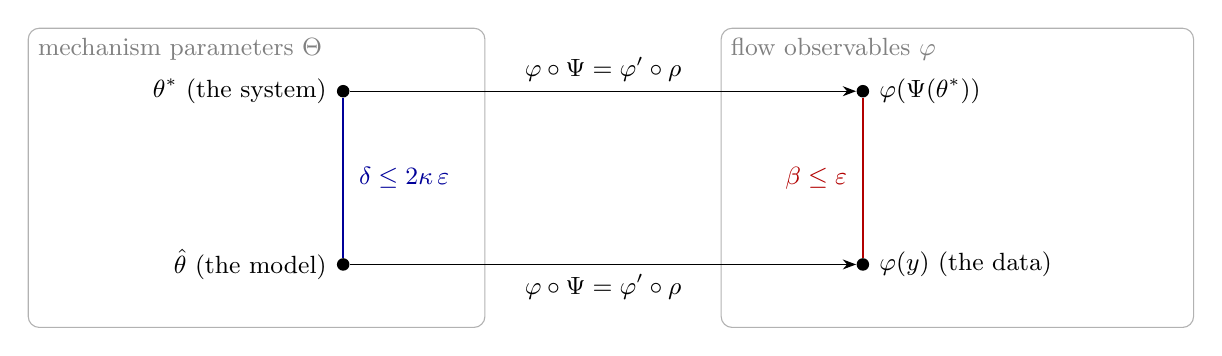
\begin{tikzpicture}[>=Stealth, font=\small]
  \draw[rounded corners, gray!60] (-2.2,-2.2) rectangle (3.6,1.6);
  \node[gray, anchor=north west] at (-2.2,1.6) {mechanism parameters $\Theta$};
  \draw[rounded corners, gray!60] (6.6,-2.2) rectangle (12.6,1.6);
  \node[gray, anchor=north west] at (6.6,1.6) {flow observables $\varphi$};
  \node[circle,fill,inner sep=1.6pt,label=left:{$\theta^{*}$ (the system)}] (ts) at (1.8,0.8) {};
  \node[circle,fill,inner sep=1.6pt,label=left:{$\hat\theta$ (the model)}] (th) at (1.8,-1.4) {};
  \node[circle,fill,inner sep=1.6pt,label=right:{$\varphi(\Psi(\theta^{*}))$}] (ps) at (8.4,0.8) {};
  \node[circle,fill,inner sep=1.6pt,label=right:{$\varphi(y)$ (the data)}] (py) at (8.4,-1.4) {};
  \draw[->] (ts) -- node[above]{$\varphi\circ\Psi=\varphi'\circ\rho$} (ps);
  \draw[->] (th) -- node[below]{$\varphi\circ\Psi=\varphi'\circ\rho$} (py);
  \draw[thick, red!70!black] (ps) -- node[left, xshift=-2pt]{$\beta\le\varepsilon$} (py);
  \draw[thick, blue!60!black] (ts) -- node[right, xshift=2pt]{$\delta\le 2\kappa\,\varepsilon$} (th);
\end{tikzpicture}
\caption{Backward and forward error for a model selected on flow observables, in the layout of the commutative diagram of \textcite[\S2]{corless2016} (cf.\ \textcite[Fig.~1.1]{higham2002}). Left: mechanism parameters, with the system's $\theta^{*}$ and the model's $\hat\theta$. Right: the values of a flow observable, with the image of each under the binding function, which by \eqref{eq:flowobs} factors through the reduction $\rho$, and the observed value $\varphi(y)$. The red segment is the backward error $\beta$ of \eqref{eq:beta}; the blue segment is the forward error $\delta$ of \eqref{eq:forward}, bounded by $2\kappa\varepsilon$ where $\kappa$ is finite and not bounded along the kernel of $\rho$.}
\label{fig:bf}
\end{figure}

\begin{figure}[htbp]\centering
\resizebox{\textwidth}{!}{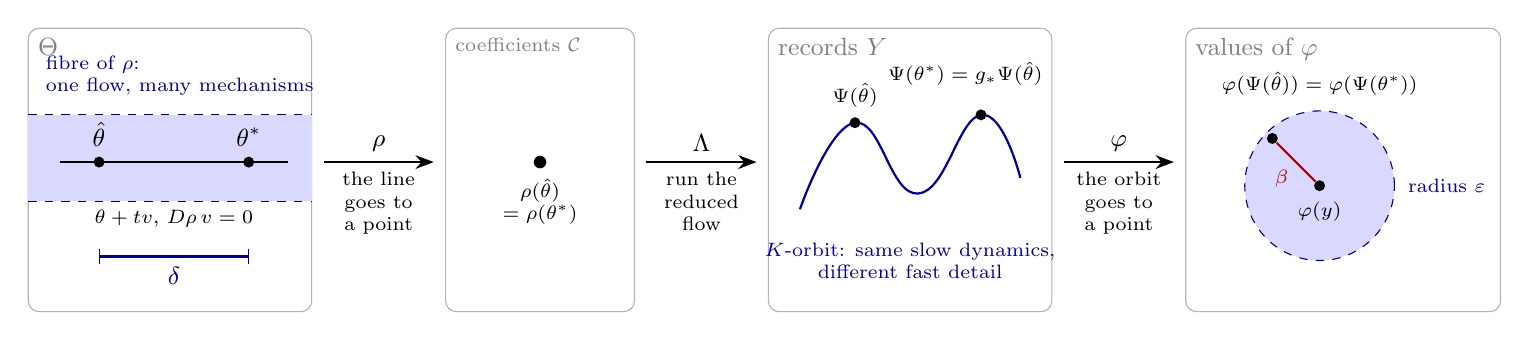
\begin{tikzpicture}[>=Stealth, font=\small]
  % Theta
  \draw[rounded corners, gray!60] (0,0) rectangle (3.6,3.6);
  \node[gray, anchor=north west] at (0,3.6) {$\Theta$};
  \fill[blue!15] (0,1.4) rectangle (3.6,2.5);
  \draw[blue!60!black, dashed] (0,1.4) -- (3.6,1.4); \draw[blue!60!black, dashed] (0,2.5) -- (3.6,2.5);
  \node[blue!60!black, anchor=south west, font=\scriptsize, align=left] at (0.1,2.62) {fibre of $\rho$:\\ one flow, many mechanisms};
  \draw[thick] (0.4,1.9) -- (3.3,1.9);
  \node[anchor=north, font=\scriptsize] at (1.85,1.42) {$\theta+tv$, $D\rho\,v=0$};
  \node[circle,fill,inner sep=1.4pt,label={[font=\small]above:$\hat\theta$}] at (0.9,1.9) {};
  \node[circle,fill,inner sep=1.4pt,label={[font=\small]above:$\theta^{*}$}] at (2.8,1.9) {};
  \draw[thick, blue!60!black] (0.9,0.7) -- node[below]{$\delta$} (2.8,0.7);
  \draw[blue!60!black] (0.9,0.6) -- (0.9,0.8); \draw[blue!60!black] (2.8,0.6) -- (2.8,0.8);
  % C
  \draw[rounded corners, gray!60] (5.3,0) rectangle (7.7,3.6);
  \node[gray, anchor=north west, font=\scriptsize] at (5.3,3.6) {coefficients $\mathcal{C}$};
  \node[circle,fill,inner sep=1.6pt,label={[font=\scriptsize, align=center]below:$\rho(\hat\theta)$\\$=\rho(\theta^{*})$}] at (6.5,1.9) {};
  % Y
  \draw[rounded corners, gray!60] (9.4,0) rectangle (13.0,3.6);
  \node[gray, anchor=north west] at (9.4,3.6) {records $Y$};
  \draw[thick, blue!60!black] plot[smooth, tension=0.8] coordinates {(9.8,1.3) (10.5,2.4) (11.3,1.5) (12.1,2.5) (12.6,1.7)};
  \node[blue!60!black, anchor=north, font=\scriptsize, align=center] at (11.2,1.0) {$K$-orbit: same slow dynamics,\\ different fast detail};
  \node[circle,fill,inner sep=1.4pt,label={[font=\scriptsize]above:$\Psi(\hat\theta)$}] at (10.5,2.4) {};
  \node[circle,fill,inner sep=1.4pt] at (12.1,2.5) {};
  \node[anchor=south, font=\scriptsize] at (11.9,2.75) {$\Psi(\theta^{*})=g_*\Psi(\hat\theta)$};
  % values
  \draw[rounded corners, gray!60] (14.7,0) rectangle (18.7,3.6);
  \node[gray, anchor=north west] at (14.7,3.6) {values of $\varphi$};
  \draw[blue!60!black, dashed, fill=blue!15] (16.4,1.6) circle (0.95);
  \node[blue!60!black, anchor=west, font=\scriptsize] at (17.4,1.6) {radius $\varepsilon$};
  \node[circle,fill,inner sep=1.4pt,label={[font=\scriptsize]below:$\varphi(y)$}] (py) at (16.4,1.6) {};
  \node[circle,fill,inner sep=1.4pt] (pp) at (15.8,2.2) {};
  \node[anchor=south, font=\scriptsize] at (16.4,2.62) {$\varphi(\Psi(\hat\theta))=\varphi(\Psi(\theta^{*}))$};
  \draw[thick, red!70!black] (py) -- node[below left, xshift=1pt, yshift=1pt, font=\scriptsize]{$\beta$} (pp);
  % arrows
  \draw[->, thick] (3.75,1.9) -- node[above]{$\rho$} node[below, font=\scriptsize, align=center, text width=1.5cm]{the line goes to a point} (5.15,1.9);
  \draw[->, thick] (7.85,1.9) -- node[above]{$\Lambda$} node[below, font=\scriptsize, align=center, text width=1.5cm]{run the reduced flow} (9.25,1.9);
  \draw[->, thick] (13.15,1.9) -- node[above]{$\varphi$} node[below, font=\scriptsize, align=center, text width=1.5cm]{the orbit goes to a point} (14.55,1.9);
\end{tikzpicture}}
\caption{The factorisation \eqref{eq:factor} and the Proposition. Left: mechanism parameters $\Theta$, with a line inside a fibre of the reduction $\rho$ through the model's $\hat\theta$ and the system's $\theta^{*}$. Second box: the flow coefficients $\mathcal{C}$; $\rho$ sends the whole line to one point. Third box: records; $\Lambda$ runs the reduced flow, and the mechanisms on the line produce laws that differ only in fast detail, one $K$-orbit. Right: a flow observable sends the orbit to one point, within $\varepsilon$ of the observed value. The shaded strip is the compatible set $A_\varepsilon(y)$, which contains the whole line; the blue segment is the forward error $\delta$, unbounded along the fibre; the red segment is the backward error $\beta$, the same at every point of the line. With $\epsilon>0$ the arrows $\rho$ and $\Lambda$ carry an $O(\epsilon)$ leak and the strip has finite length, of order the tolerance $\varepsilon$ divided by the leak.}
\label{fig:prop}
\end{figure}

\section{The critique relative to a target}
The Proposition is about $\theta$. Nobody asks about $\theta$. The authors ask whether a system is bistable, where a coupling sits relative to a threshold, which regions are excitable, whether a flow is robust to a class of changes; each is a functional of $\theta$, and the question is which functionals the flow identifies. This section restates the critique so that it answers that question, in three steps, each worked on one small case.

\subsection{The small case}
Take a slow variable $x$ and a fast one $y$,
\begin{equation}
\dot x=\varepsilon_0 x-b\,xy,\qquad \dot y=-\gamma\,(y-a x^2),\qquad \gamma\gg1,
\label{eq:small}
\end{equation}
so $\theta=(\varepsilon_0,a,b,\gamma)$. The fast variable relaxes to $y\approx ax^2$ and the slow equation closes as $\dot x\approx\varepsilon_0x-ab\,x^3$: a pitchfork with coefficients $c(\theta)=(\varepsilon_0,\,ab)$. The record is $x$ alone. The reduction is $\rho(\theta)=(\varepsilon_0,ab)$, its fibres are the sets $\{\varepsilon_0=\text{const},\ ab=\text{const}\}$ with $\gamma$ free, and here $\epsilon=1/\gamma$, so $\epsilon=0$ is the limit $\gamma\to\infty$. The leak has two parts: the transient of length $1/\gamma$ before $y$ reaches the slow manifold, and a persistent correction on it. Writing $y=ax^2+\eta$ and requiring invariance, $-\gamma\eta=2ax\,\dot x_0$ with $\dot x_0=\varepsilon_0x-abx^3$, so
\begin{equation}
\dot x=\dot x_0\,\Bigl(1+\frac{2ab\,x^2}{\gamma}\Bigr)+O(\gamma^{-2}),
\label{eq:correction}
\end{equation}
a state-dependent change of speed that leaves orbits and fixed points in place. In coefficients it is a shift of the cubic term by $2ab\varepsilon_0/\gamma$ and a new quintic term $-2a^2b^2x^5/\gamma$.

\subsection{Target functionals and the identified algebra}
Let $g:\Theta\to G$ be a \emph{target functional}, the quantity a claim is about. Say that $g$ is \emph{identified by flow observables} if $g(\theta)=g(\theta')$ whenever $\theta$ and $\theta'$ are observationally equivalent with respect to every flow observable. Write
\begin{equation}
\mathcal{A}_\rho=\{\,g=g'\circ\rho\ :\ g':\mathcal{C}\to G\,\}
\label{eq:algebra}
\end{equation}
for the functionals that factor through the reduction; I call it the \emph{identified algebra} of $\rho$.
\begin{proposition}[identification relative to a target]
Let $\epsilon=0$ and let $\Lambda$ be injective (at $\epsilon=0$ every statistic is a flow observable, so this is the whole hypothesis). Then $g$ is identified by flow observables if and only if $g\in\mathcal{A}_\rho$. Locally: at a point near which $D\rho$ and $[D\rho;\,Dg]$ have constant rank, $g$ is locally identified if and only if $Dg\,v=0$ for every $v\in\ker D\rho$ on a neighbourhood.
\end{proposition}
\begin{proof}
If $g=g'\circ\rho$ and $\theta,\theta'$ are observationally equivalent, then $\Lambda(\rho(\theta))=\Lambda(\rho(\theta'))$, so by injectivity $\rho(\theta)=\rho(\theta')$ and $g(\theta)=g(\theta')$. Conversely, if $g\notin\mathcal{A}_\rho$ there are $\theta,\theta'$ in one fibre with $g(\theta)\neq g(\theta')$; then $\Psi(\theta)=\Lambda(\rho(\theta))=\Lambda(\rho(\theta'))=\Psi(\theta')$, the record laws are equal, so $\theta,\theta'$ are observationally equivalent with respect to every statistic and $g$ is not identified. For the local form, constant rank of $D\rho$ makes the fibre through $\theta$ locally a connected submanifold with tangent space $\ker D\rho$, and $g$ is constant on it iff $Dg$ annihilates $\ker D\rho$ along it; the pointwise condition does not suffice ($\rho=\theta_1$, $g=\theta_2^2$ at $0$). \hfill⟦HAND, checked by an independent referee pass 2026-11-19⟧
\end{proof}
In the small case $\mathcal{A}_\rho$ is the functions of $(\varepsilon_0,ab)$: the sign of $\varepsilon_0$, the product $ab$, the number and position of fixed points are identified; $\gamma$, $a$ and $b$ separately are not, away from $ab=0$ where the fibre is not a manifold. Under injectivity of $\Lambda$ the proposition says only that identified means constant on the fibres of $\Psi$, which is standard; its use is the computation it licenses on $D\rho$. The critique of \S3 is the special case $g=\mathrm{id}$, and it is the case nobody asserts. What the Proposition now does is sort claims: a claim is a flow claim if its functional is in $\mathcal{A}_\rho$, a mechanism claim otherwise, and the sorting is a computation on $D\rho$, not a matter of how the claim is worded.

\subsection{Admissible sets and families of reductions}
Two things cut the fibre in practice. Parts are measured independently of the dynamics, the connectome above all, which restricts $\theta$ to an \emph{admissible set} $\Theta_{\mathrm{adm}}=\{h(\theta)=0\}$; and records come from several conditions, a sweep of a coupling, a task, a lesion, a second patient, each with its own reduction $\rho_k$, $k=1,\dots,K$, because the slow manifold and its coefficients depend on the condition. The relevant fibre is then
\begin{equation}
\mathcal{F}(\theta)=\Theta_{\mathrm{adm}}\cap\bigcap_{k=1}^{K}\rho_k^{-1}\bigl(\rho_k(\theta)\bigr),
\label{eq:jointfibre}
\end{equation}
and the identified algebra is the functionals constant on $\mathcal{F}$.
\begin{proposition}[rank condition]
Let $\epsilon=0$, let $\theta\in\Theta_{\mathrm{adm}}$ be a point near which the stacked matrix $R=[D\rho_1;\dots;D\rho_K;Dh]$ and the augmented matrix $[R;Dg]$ have constant rank, and let each reduced information matrix $I_{\mathcal{C},k}$ be nonsingular there. Then $g$ is locally identified by flow observables across the conditions, given the constraints, if and only if
\begin{equation}
Dg\in\operatorname{rowspan}\begin{bmatrix}D\rho_1\\ \vdots\\ D\rho_K\\ Dh\end{bmatrix}\quad\text{on a neighbourhood of }\theta.
\label{eq:rank}
\end{equation}
\end{proposition}
\begin{proof}
Under constant rank, $\mathcal{F}$ is locally a connected submanifold with tangent space $\ker R$, and $g$ is locally constant on it iff $Dg$ annihilates $\ker R$ along it, iff $Dg$ lies in the row span of $R$ there; the ``only if'' needs constant rank of $R$ alone. Observational equivalence here is joint: the same $\theta'$ equivalent to $\theta$ in every condition. Nonsingularity of the $I_{\mathcal{C},k}$ is what lets $\sum_k D\rho_k^{\top}I_{\mathcal{C},k}D\rho_k$ be replaced by the stacked $D\rho_k$, since the two then have the same row span; injectivity of $\Lambda_k$ does not give this ($c\mapsto$ a law with parameter $c^3$). The condition is of Rothenberg's type \parencite{rothenberg1971}; his theorems concern $\theta$ itself, and the row-span form for a functional is the estimability criterion. \hfill⟦HAND, referee-checked 2026-11-19⟧ \CHECK{confirm whether Rothenberg 1971 states the functional form}
\end{proof}
In the small case, add a second condition in which a known input $u$ drives the fast variable, $\dot y=-\gamma(y-ax^2-u)$. The slow equation becomes $\dot x=(\varepsilon_0-bu)\,x-ab\,x^3$, so $\rho_2(\theta)=(\varepsilon_0-bu,\,ab)$, and the two conditions together identify $b=u^{-1}[\varepsilon_0-(\varepsilon_0-bu)]$, linearly and with sign, and then $a$ from the product, for $u\neq0$ and $b\neq0$: the stacked Jacobian has rows $(1,0,0,0)$, $(0,b,a,0)$, $(1,0,-u,0)$, $(0,b,a,0)$, of rank three with kernel the $\gamma$ axis. This presumes that the flow observables recover the linear and the cubic coefficient in each condition; fixed-point positions alone give $a$ and $\varepsilon_0/b$ and leave the time rescaling $(\varepsilon_0,b)\mapsto\lambda(\varepsilon_0,b)$ invisible, so timing observables, relaxation rates or autocorrelations, are needed. The family cuts the fibre in every direction that enters some reduced flow. At leading order it never reaches $\gamma$: the rate of slaving enters no $\rho_k$, and enters the reduced flow only at $O(1/\gamma)$ through \eqref{eq:correction}; the ways to it are an independent measurement, a row of $Dh$, or a statistic that reads the leak. This is Objection R1 of the earlier draft made exact. The parts can warrant the mechanism, and \eqref{eq:rank} says which parts, in which conditions, warrant which functionals.

\subsection{Finite-sample resolution}
With $\epsilon>0$ the leak makes every direction identified in principle, and the question is at what record length. The Fisher information of a record of length $T$ splits, by \eqref{eq:fisher}, into a stiff block that grows with $T$ along $\mathcal{C}$ and a leak block along $\ker D\rho$ that also grows with $T$, at rate $O(\epsilon^2)$. In the stiff block the condition number is finite and a functional in $\mathcal{A}_\rho$ is resolved at the parametric rate. In a leak direction $v$ with $\beta_v=O(\epsilon)$, resolving it at tolerance $\varepsilon$ needs the sampling deviation of $\varphi$ below $\beta_v$, which for a statistic with variance of order $\sigma^2/T$ is
\begin{equation}
T\ \gtrsim\ \sigma^2/\beta_v^{2}. \tag{heuristic}
\label{eq:samplecomplexity}
\end{equation}
⟦HAND, order of magnitude; the rate below referee-checked 2026-11-19⟧ Where the information sits matters more than the constant. In the small case $\gamma$ enters through the initial transient and through the change of slow speed \eqref{eq:correction}. A deterministic record that settles at a fixed point carries $O(1)$ information about $\gamma$, as it does about every parameter. A stationary record with process noise $\sigma$ on $x$ carries $O(T)$: by Girsanov on the drift, $I_\gamma(T)\approx (T/\sigma^2\gamma^4)\,\mathbb{E}_\pi[(2abx^2\dot x_0+ab\sigma^2x)^2]$, consistent with \eqref{eq:samplecomplexity} at $\epsilon=1/\gamma$, and the $\gamma$-specific part has density $\propto x^4\dot x_0^2$, zero at the fixed points and largest where the slow flow is fast. Near a single fixed point what information there is arrives through the relaxation rate $2\varepsilon_0(1+2\varepsilon_0/\gamma)$ and is confounded with $\varepsilon_0$; $\gamma$ separates only through excursions over which the speed factor varies, of which transitions between basins are the largest. So the leak observables that can resolve the fibre in a long record are those that sample fast segments of the slow flow, the dwell and transition structure and the relaxation after each switch above all, and not transients in general. The framework's papers report no $\varepsilon$ and no $T$-dependence against which to read this.

\subsection{Class-level claims as tests}
Many of the authors' functionals are discrete: bistable or not, which bifurcation at onset, how many basins. A discrete $g\in\mathcal{A}_\rho$ is identified, and estimating it from a finite record is a classification with error rates, which is a hypothesis test: a statistic, a null that is the model's own flow with the class removed, and a power. The companion essay runs such tests for three statistics against phase-randomised and autoregressive nulls. What is identified is the class; the mechanism that realises it is still the fibre.

\subsection{The fibre as content}
The framework's claim in \S2.2, that the degeneracy manifold confers robustness, is a claim about $\ker D\rho$: perturb $\theta$ along the fibre and the flow does not move, perturb it transversally and it does. That is a prediction, and it is testable by acting on $\theta$, in models directly and in brains by lesion or stimulation, never by one record. Weak invariance is the same claim for a coarser reduction, the map to the flow's topological type. In the small case the prediction is that changing $\gamma$ changes nothing in the long-run distribution of $x$ while changing $a$ at fixed $b$ does. Read this way the many-to-one is not the framework's embarrassment but its empirical content, and the test of the framework is the test of its predicted kernel.

\subsection{The authors' claims, classified}
Table~\ref{tab:claims} places the published claims. The status column uses the three grades: identified (the functional is in $\mathcal{A}_\rho$), identified given constraints (it satisfies \eqref{eq:rank} with the stated parts and conditions), not identified by the flow. The last column says what would move the status.
\begin{table}[htbp]\centering\small
\begin{tabular}{@{}p{3.6cm}p{3.9cm}p{3.1cm}p{4.4cm}@{}}
\toprule
Claim & Target functional $g$ & Status & What would settle it \\
\midrule
Jirsa 2020: the flow is fixed by few coefficients & $g=c=\rho(\theta)$ & identified, by definition & the separation hypothesis for the statistics used \\
Jirsa 2020: degeneracy confers robustness & a statement about $\ker D\rho$ & a prediction, untested as stated & perturbation along and across the fibre (\S4.6) \\
Jirsa 2020: strong vs weak invariance & $\beta_v=0$ vs $\beta_v\le\varepsilon$ along the fibre & gradable only with a tolerance & report $\varepsilon$ and $T$ \\
Fousek et al.\ 2024: a bistable regime at $(G,\sigma)$ \parencite{fousek2024} & the number of basins, discrete, in $\mathcal{A}_\rho$ & identified; tested against surrogates in the companion essay & power of the test at the sizes used \\
Fousek et al.\ 2024: in-strength organises the basins & that $c$ depends on $W$ through its row sums & a claim about $\rho$; tested by rewiring in the companion essay, results mixed & a perturbation that holds $\lambda_1(W)$ fixed \\
Fousek et al.\ 2024: symmetry breaking is the mechanism & the generating process & not identified by the flow & a leak observable or an intervention \\
Virtual epileptic patient: per-region excitability \parencite{jirsa2017,wang2023} & a coefficient of the node normal form, with the connectome in $\Theta_{\mathrm{adm}}$ & identified given constraints, with reported uncertainty \parencite{hashemi2024} & the trial outcome, which tests the intervention on it \\
\bottomrule
\end{tabular}
\caption{The framework's published claims placed in the classification of \S4. The companion essay supplies the tests in rows four and five.}
\label{tab:claims}
\end{table}

\section{What is missing: a skeleton}
The reformulation names what a complete assessment needs. Each item is stated, with what would settle it and whether a generic-case method is known. None is solved here, and whether each can be solved in the generic case is the question this skeleton is for.
\begin{enumerate}[label=O\arabic*.,leftmargin=2.6em]
\item \emph{The identified algebra of a given pipeline.} It is a computation on $D\rho$, and $\rho$ is only available where the reduction can be carried out: near an instability by centre-manifold reduction, elsewhere numerically. Jirsa's global case, symmetry breaking away from any instability, has no general method for $D\rho$ that I know of. Open.
\item \emph{The rank condition across conditions.} It needs the $\rho_k$ and $Dh$. When a family of conditions spans the directions a claim needs is a question of experimental design for identifiability, with an existing literature for ODE models \CHECK{structural identifiability, Chis et al.; cite} and, so far as I know, none for reduced flows. Open.
\item \emph{Finite-sample resolution.} The stiff Fisher block can be estimated by simulation-based inference, which the framework's own group uses \parencite{hashemi2024}; what is missing is its use to report a condition number and a tolerance, and the recurrence qualification of \S4.4 as a statement with constants. Addressable with existing tools; not done.
\item \emph{Class tests with power.} Surrogate nulls exist; their power at the record lengths used is not reported. Addressable; not done.
\item \emph{The fibre as prediction.} Perturbation along and across $\ker D\rho$ is routine in models and available in brains only through lesion and stimulation data. Whether the framework's robustness claim has been tested this way anywhere I have not checked. Open.
\item \emph{A geometry for the gap.} The Fisher information is a degenerate metric on $\Theta$ whose null directions are exactly $\ker D\rho$ at $\epsilon=0$; the quotient $\Theta/K$ with the pushed-forward metric is the model manifold of the flow, and the stiff--sloppy spectrum is its curvature and extent \parencite{machta2013}. The backward error is a distance in the quotient; the forward error is a distance in $\Theta$ that the Fisher metric does not see; the condition number is their ratio. The intuition to keep is that information geometry may give the gap its proper expression, as the difference between the Fisher metric the data induce on $\Theta$ and the metric a mechanistic claim needs there, an intervention metric in which moving along the fibre is not free. Unformed; recorded so that it is not lost. \CHECK{owners to read: Amari; Transtrum, Machta and Sethna on model manifolds}
\end{enumerate}

\subsection{Limits}
Everything here assumes the slow--fast split the framework asserts; where it fails, so does the kernel, and the mechanism becomes visible in the slow observables. Proximity to an instability and time-scale separation are assumptions in the brain. The order parameters in practice are chosen, not derived, and the argument applies to whichever are used. The two propositions of \S4 are stated at $\epsilon=0$ and at regular points; the approximate grade is heuristic. Nothing here touches the normal-form claims themselves, the fixed-point analyses, or the empirical regularities the framework has found.

\section{Conclusion}
The framework says that many mechanisms give one flow and that the flow is a causal description of the brain. As a theorem about $\theta$ the first forecloses the second at the level of flow observables, and as a theorem about $\theta$ it also misses how the approach works in practice. Restated relative to a target functional, an admissible set and a family of reductions, it sorts the framework's claims into those the flow identifies, those the measured parts and the conditions identify, and those nothing in the flow identifies, and it names six things that a complete assessment needs and does not yet have. Whether those six can be supplied in the generic case is the next question, and until it is answered the question of what kind of explanation the framework gives stays open.

\printbibliography
\end{document}
